\chapter{Bayesian Inference and Classical Computational Intractability}\label{chap:classical_limits}

\section{The Predictive Model: Bayesian Networks in Astrobiology}\label{sec:predictive_model_bn}

To establish the mathematical necessity of quantum computational acceleration, we must first formalize the probabilistic framework currently deployed to characterize exoplanetary environments: the Bayesian Network. A Bayesian Network (BN) is a directed probabilistic graphical model that represents a multivariate joint probability distribution over a set of random variables through a Directed Acyclic Graph (DAG) \cite{pearl1988}. In exoplanetary astrobiology, this model functions as the primary causal inference engine, transforming sparse, noisy spectroscopic telemetry gathered across light-years into structured, probabilistic assertions regarding the habitability and biological status of distant worlds.

\notatfm{\textbf{Formal Model:} A Bayesian Network $\mathcal{B} = (\mathcal{G}, \Theta)$ factorizes a $2^N$ joint distribution into local conditional probability tables (CPTs).}
Formally, a Bayesian Network is defined as an ordered pair $\mathcal{B} = (\mathcal{G}, \Theta)$. The structural component $\mathcal{G} = (V, E)$ is a DAG in which the set of vertices $V = \{X_1, X_2, \dots, X_N\}$ represents random variables, and the directed edges $E \subseteq V \times V$ encode direct conditional causal influences. In an astrobiological retrieval model, these vertices represent planetary, geochemical, and stellar parameters: stellar spectral class, chromospheric ultraviolet (UV) flux, surface atmospheric pressure, effective equilibrium temperature, and the atmospheric volume mixing ratios of volatile species such as $\mathrm{H}_2\mathrm{O}$, $\mathrm{CO}_2$, $\mathrm{O}_2$, $\mathrm{CH}_4$, dimethyl sulfide ($\mathrm{DMS}$), or synthetic industrial pollutants such as chlorofluorocarbons ($\mathrm{CFCs}$). In this framework, while $\mathrm{DMS}$ serves as a representative volatile trace biosignature proxy motivated by tentative JWST transmission signals \cite{madhusudhan2023}, it is modeled strictly as a computational benchmark test-case, acknowledging the ongoing debate regarding potential abiotic photochemical production pathways in sub-Neptune atmospheres.

The parametric component $\Theta = \{P(X_i \mid \mathrm{Parents}(X_i)) : i \in \{1, \dots, N\}\}$ comprises the set of Conditional Probability Tables (CPTs) quantifying the local stochastic relationship of each variable conditioned on its immediate parent set in $\mathcal{G}$, denoted as $\mathrm{Parents}(X_i) = \{X_j \in V : (X_j, X_i) \in E\}$. The expressive power of a Bayesian Network derives from the Markov condition: each variable $X_i$ is conditionally independent of its non-descendants given its parents. Consequently, the complete Joint Probability Distribution (JPD) over all $N$ variables factorizes as the product of these local conditional terms:
\begin{equation}
P(X_1, X_2, \dots, X_N) = \prod_{i=1}^N P\left(X_i \mid \mathrm{Parents}(X_i)\right).
\label{eq:jpd_factorization_ch2}
\end{equation}

In astrobiological practice, this causal factorization governs the operational workflow. When space observatories---such as the James Webb Space Telescope (JWST) \cite{madhusudhan2023}---capture the transit transmission spectrum of an exoplanet, molecular absorption features are extracted and injected into the graph as observed evidence $\mathbf{E} = \mathbf{e}$. The inference engine then computes the posterior marginal distribution of unobserved latent hypotheses through Bayes' theorem:
\begin{equation}
P(\mathrm{Biosphere} \mid \mathbf{E} = \mathbf{e}) = \frac{P(\mathbf{E} = \mathbf{e} \mid \mathrm{Biosphere}) P(\mathrm{Biosphere})}{P(\mathbf{E} = \mathbf{e})}.
\label{eq:bayes_theorem_inversion}
\end{equation}
This allows astronomers to perform abductive causal reasoning, updating the likelihood of an unobservable biological or technological source based on observable atmospheric evidence.

\section{Exact Inference Techniques: Combinatorial Explosion and the Treewidth Limit}\label{sec:exact_inference_treewidth}

Once the topology $\mathcal{G}$ and parameters $\Theta$ are defined, computation focuses on evaluating inferential queries. In astrobiology, this translates to determining the exact posterior probability of a target biological indicator $X_Q \in V$ conditioned on observed evidence $\mathbf{E} = \mathbf{e}$. Computing this posterior requires marginalizing (summing out) the set of unobserved latent nuisance parameters $Y = V \setminus (\{X_Q\} \cup \mathbf{E})$:
\begin{equation}
P(X_Q \mid \mathbf{E} = \mathbf{e}) = \frac{\sum_{Y} \prod_{i=1}^N P\left(X_i \mid \mathrm{Parents}(X_i)\right)}{\sum_{X_Q, Y} \prod_{i=1}^N P\left(X_i \mid \mathrm{Parents}(X_i)\right)}.
\label{eq:exact_marginal_query_ch2}
\end{equation}

\subsection{Variable Elimination and Intermediate Factor Scopes}
The fundamental classical algorithm for exact inference is \emph{Variable Elimination (VE)}. VE computes the summation in Equation \eqref{eq:exact_marginal_query_ch2} by iteratively distributing sums over products according to a predefined elimination ordering $\pi$. Each variable elimination step marginalizes out a latent variable $Y_j$ by computing an intermediate factor:
\begin{equation}
\tau_j(S_j) = \sum_{Y_j} \prod_{\phi_k \in \Phi_j} \phi_k,
\label{eq:ve_intermediate_factor}
\end{equation}
where $\Phi_j$ is the set of active factors whose scope contains $Y_j$, and $S_j = \left(\bigcup_{\phi_k \in \Phi_j} \mathrm{Scope}[\phi_k]\right) \setminus \{Y_j\}$ is the scope of the generated factor. 

The spatial memory required to store $\tau_j$ in Random Access Memory (RAM) scales exponentially with the cardinality of its scope:
\begin{equation}
\mathcal{M}(\tau_j) = \mathcal{O}\left(d^{|S_j|}\right),
\label{eq:factor_memory_scaling}
\end{equation}
where $d$ is the maximum domain cardinality of the discrete variables (e.g., discretization bins for gas mixing ratios). If the elimination ordering induces an intermediate factor containing 40 variables, storing $\tau_j$ for binary variables ($d=2$) requires $2^{40}$ floating-point values---exceeding 8 terabytes of RAM for a single computational step.

\subsection{The Junction Tree Algorithm and the Treewidth Ceiling}
To support arbitrary simultaneous queries across the entire network without re-executing Variable Elimination, classical systems compile the DAG into a secondary tree-structured graphical model via the \emph{Junction Tree Algorithm (JTA)}. The JTA compiler executes four deterministic structural phases:
\begin{enumerate}
    \item \textbf{Moralization:} The directed graph $\mathcal{G}$ is converted into an undirected graph $\mathcal{G}_M$ by adding an undirected edge between all pairs of nodes that share a common child (marrying parents) and subsequently dropping all edge directions.
    \item \textbf{Triangulation:} Chordal edges are added to $\mathcal{G}_M$ such that every cycle of length greater than or equal to 4 possesses a chord (an edge connecting two non-consecutive vertices of the cycle), yielding a triangulated chordal graph $\mathcal{G}_T$.
    \item \textbf{Clique Tree Construction:} The maximal cliques $\mathcal{C} = \{C_1, C_2, \dots, C_k\}$ of $\mathcal{G}_T$ are identified and organized into a Junction Tree $\mathcal{T} = (\mathcal{C}, \mathcal{S})$, where separator sets $S_{ij} = C_i \cap C_j$ connect adjacent cliques satisfying the Running Intersection Property (RIP).
    \item \textbf{Belief Propagation:} Potentials $\psi(C_i)$ are initialized by assigning each CPT factor to a containing clique, followed by two-pass message passing (Shafer-Shenoy or Hugin architecture) across separator sets.
\end{enumerate}

\notatfm{\textbf{Treewidth Ceiling:} Classical exact inference via Junction Tree is bounded by $\mathcal{O}(N \cdot d^{w+1})$. Dense photochemical loops force $w \to N$, saturating RAM.}
The computational tractability of the Junction Tree algorithm is strictly governed by a topological metric: the \emph{treewidth} ($w$) of the moralized, triangulated graph. The treewidth is defined as the size of the largest maximal clique minus one:
\begin{equation}
w \equiv \max_{C_i \in \mathcal{C}} |C_i| - 1.
\label{eq:treewidth_definition}
\end{equation}
Because the algorithm must compile joint potential tables for every maximal clique, the spatial and temporal complexity of exact inference is bounded by:
\begin{equation}
\mathcal{C}_{\mathrm{exact}} = \mathcal{O}\left(N \cdot d^{w+1}\right).
\label{eq:jta_treewidth_bound_ch2}
\end{equation}

\input{figures/2.classical_limits/figure_junction_tree.tex}

In an exoplanetary atmosphere, dense photochemical cycling renders the network topologically non-sparse. Photochemical reactions link atmospheric species into closed cycles (e.g., the catalytic destruction of methane by hydroxyl radicals, coupled to stellar UV photolysis and volcanic outgassing). During moralization, marrying multiple parents across these feedback loops introduces dense fill-in edges. As network connectivity approaches a complete graph, the treewidth $w$ approaches $N - 1$. 

Under this condition, the memory requirement scales as $\mathcal{O}(d^N)$, precipitating a catastrophic spatial failure. For a realistic photochemical network with $N = 50$ species, compiling the Junction Tree demands memory on the order of exabytes. This combinatorial wall is an inescapable consequence of complexity theory: Cooper (1990) established by polynomial reduction from 3-SAT that exact probabilistic inference in Bayesian belief networks is NP-hard \cite{cooper1990}.

\section{Stochastic Inference: Markov Chain Monte Carlo and Asymptotic Slowdown}\label{sec:stochastic_inference_mcmc}

Confronting the exponential spatial ceiling $\mathcal{O}(N \cdot d^{w+1})$ of exact algorithms, classical astrobiological modeling uniformly abandons exact algebraic calculation in favor of stochastic approximation. These methods bypass the compilation of multi-dimensional clique tensors by generating empirical trajectories through the state space. The dominant classical sampling architecture is Markov Chain Monte Carlo (MCMC), implemented primarily through the Metropolis-Hastings algorithm and Gibbs sampling.

\subsection{Metropolis-Hastings Formulation on Discrete Causal Graphs}
Mathematically, MCMC constructs an ergodic, discrete-time Markov chain $\{X^{(t)}\}_{t=0}^M$ over the state space $\mathcal{S} = \{0, 1\}^N$. The transition dynamics are defined by a stochastic kernel $T(\mathbf{x} \to \mathbf{x}')$ engineered to converge to a unique stationary equilibrium distribution $\pi(\mathbf{x})$. To perform Bayesian inference, this stationary distribution must match the posterior distribution conditioned on observational evidence: $\pi(\mathbf{x}) \equiv P(\mathbf{x} \mid \mathbf{E} = \mathbf{e}) \propto P(\mathbf{x}, \mathbf{e})$. This convergence is guaranteed if the transition kernel satisfies the detailed balance condition:
\begin{equation}
\pi(\mathbf{x}) T(\mathbf{x} \to \mathbf{x}') = \pi(\mathbf{x}') T(\mathbf{x}' \to \mathbf{x}), \quad \forall \mathbf{x}, \mathbf{x}' \in \mathcal{S}.
\label{eq:detailed_balance_ch2}
\end{equation}

In the Metropolis-Hastings framework, a candidate state $\mathbf{x}'$ is generated from a proposal distribution $q(\mathbf{x}' \mid \mathbf{x})$ by randomly selecting a non-evidence variable $X_j \notin \mathbf{E}$ and flipping its binary assignment ($x'_j = 1 - x_j$, transitioning at Hamming distance 1). For symmetric proposals where $q(\mathbf{x}' \mid \mathbf{x}) = q(\mathbf{x} \mid \mathbf{x}')$, the candidate state is accepted with probability:
\begin{equation}
\alpha(\mathbf{x}, \mathbf{x}') = \min\left(1, \frac{\pi(\mathbf{x}')}{\pi(\mathbf{x})}\right) = \min\left(1, \frac{P(\mathbf{x}', \mathbf{e})}{P(\mathbf{x}, \mathbf{e})}\right).
\label{eq:metropolis_hastings_acceptance_ch2}
\end{equation}
If accepted, the chain advances to $\mathbf{x}^{(t+1)} = \mathbf{x}'$; otherwise, it remains at $\mathbf{x}^{(t+1)} = \mathbf{x}^{(t)}$.

The expectation value $\mu = \mathbb{E}[f(X)]$ of an astrobiological query function $f: \mathcal{S} \to \{0, 1\}$ (e.g., an indicator for habitability) is estimated by the empirical time-average over $M$ generated samples:
\begin{equation}
\hat{\mu}_M = \frac{1}{M} \sum_{t=1}^M f\left(X^{(t)}\right).
\label{eq:empirical_mcmc_estimator}
\end{equation}

\subsection{Asymptotic Slowdown and the Central Limit Theorem}
While MCMC requires minimal memory---storing only the current configuration $\mathbf{x}^{(t)}$ in RAM ($\mathcal{O}(N)$ space)---it trades the spatial barrier for a severe temporal barrier. Successive states in a Markov chain are not independent; they exhibit temporal serial correlation. According to the Markov Chain Central Limit Theorem, the statistical variance of $\hat{\mu}_M$ decays as:
\begin{equation}
\mathrm{Var}(\hat{\mu}_M) \approx \frac{\sigma_0^2}{M} \cdot \tau_{\mathrm{int}},
\label{eq:clt_mcmc_variance_ch2}
\end{equation}
where $\sigma_0^2 = \mathrm{Var}_{\pi}[f(X)]$ is the static variance under the stationary distribution, and $\tau_{\mathrm{int}}$ is the integrated autocorrelation time:
\begin{equation}
\tau_{\mathrm{int}} \equiv 1 + 2 \sum_{k=1}^\infty \rho(k),
\label{eq:integrated_autocorrelation_time}
\end{equation}
with $\rho(k) = \mathrm{Cov}(f(X^{(t)}), f(X^{(t+k)})) / \sigma_0^2$ denoting the normalized autocorrelation at lag $k$. 

Consequently, the standard error (root-mean-square error) of the estimator decays as:
\begin{equation}
\sigma(\hat{\mu}_M) = \mathcal{O}\left(\frac{1}{\sqrt{M}}\right).
\label{eq:mcmc_asymptotic_rate}
\end{equation}

\notatfm{\textbf{Quadratic Penalty:} MCMC error decays as $\mathcal{O}(1/\sqrt{M})$. Gaining one digit of precision requires multiplying CPU runtime by $100\times$.}
This $\mathcal{O}(1/\sqrt{M})$ rate imposes an unyielding quadratic computational penalty: gaining an additional decimal digit of precision in posterior likelihood ($\epsilon \to 0.1\epsilon$) requires a hundredfold increase in sample size ($M \to 100M$). Gaining two decimal digits requires a $10,000\times$ increase in compute time.

Fundamentally, Dagum and Luby (1993) established that approximating probabilistic inference in Bayesian networks within a specified error margin $\epsilon$ is itself NP-hard \cite{dagum1993}. Stochastic sampling does not bypass theoretical complexity; it merely reframes an exponential spatial problem into an asymptotically intractable temporal problem.

\subsection{Multimodal Topologies and Mixing Time Stagnation}
This temporal drag is exacerbated when the probability landscape is multimodal \cite{mackay2003}. In astrobiology, competing planetary regimes (e.g., an abiotic volcanic world with thick $\mathrm{CO}_2$ vs. a water-rich biotic Hycean world) represent distinct local probability maxima separated by wide valleys of near-zero likelihood. The mixing time $t_{\mathrm{mix}}(\epsilon)$ required for the Markov chain to approach within total variation distance $\epsilon$ of $\pi$ scales inversely with the spectral gap $\gamma = 1 - \lambda_2$ of the transition matrix:
\begin{equation}
t_{\mathrm{mix}}(\epsilon) \le \frac{1}{\gamma} \ln\left(\frac{1}{\epsilon \cdot \pi_{\min}}\right).
\label{eq:spectral_gap_mixing_time}
\end{equation}
When transition barriers between modes have probability $\ll 1$, the spectral gap $\gamma$ vanishes exponentially, trapping the chain in a single local mode for millions of steps and producing severely biased, unrepresentative posteriors.

\section{Structural Failure Modes: Discretization, Rejection Sampling, and Structure Learning}\label{sec:structural_failure_modes}

Beyond exact treewidth bounds and MCMC convergence slowdowns, classical inference suffers from three additional structural failure modes when applied to exoplanetary systems.

\subsection{Continuous Variable Discretization Blowup}
Astronomical observations are continuous physical measurements: surface temperature in Kelvin, stellar extreme ultraviolet (EUV) flux in $\mathrm{erg}\,\mathrm{s}^{-1}\,\mathrm{cm}^{-2}$, and gas column densities in $\mathrm{mol}\,\mathrm{cm}^{-2}$. Because exact continuous inference is computationally intractable outside of linear Gaussian networks, classical models discretize each continuous dimension into $k$ discrete bins.

Friedman and Goldszmidt (1996) proved that discretizing continuous attributes in Bayesian networks induces an exponential parameter explosion \cite{friedman1996}. For a variable $X_i$ with $p = |\mathrm{Parents}(X_i)|$ continuous parents, the number of independent conditional probability parameters required scales as:
\begin{equation}
|\Theta_{X_i}| = (k - 1) \cdot k^p = \mathcal{O}\left(k^{p+1}\right).
\label{eq:discretization_cpt_explosion}
\end{equation}
This imposes an intractable trade-off: coarse discretization ($k = 2$ or $3$) erases critical non-linear planetary thresholds (such as the narrow temperature window for liquid water condensation), while fine discretization ($k \ge 10$) causes CPT sizes to overwhelm classical memory hardware.

\subsection{Rejection Sampling and L'Ecuyer's Relative Error Divergence}
To evaluate conditional queries, classical algorithms frequently implement Rejection Sampling: generating configurations from a prior distribution and discarding those inconsistent with observed evidence $\mathbf{e}$. When inferring ultra-rare events---such as an industrial technosignature with prior probability $p \approx 10^{-6}$---rejection sampling suffers from severe asymptotic variance instability.

\notatfm{\textbf{L'Ecuyer's Theorem:} Relative error diverges as $\mathrm{RE} = \sqrt{\frac{1-p}{M p}} \to \infty$. Rare events ($p \to 0$) become statistically invisible to classical samplers.}
As formalized by L'Ecuyer et al.~(2010) in rare-event simulation theory \cite{lecuyer2010}, evaluating an estimator requires measuring its Relative Error ($\mathrm{RE}$):
\begin{equation}
\mathrm{RE}(\hat{p}_M) \equiv \frac{\sigma(\hat{p}_M)}{\mathbb{E}[\hat{p}_M]} = \frac{\sqrt{\frac{p(1-p)}{M}}}{p} = \sqrt{\frac{1-p}{M \cdot p}}.
\label{eq:lecuyer_theorem_ch2}
\end{equation}
As the prior probability of the target phenomenon tends to zero, the relative variance diverges toward infinity:
\begin{equation}
\lim_{p \to 0} \mathrm{RE}(\hat{p}_M) = \lim_{p \to 0} \frac{1}{\sqrt{M \cdot p}} = \infty.
\label{eq:lecuyer_limit_divergence}
\end{equation}

To bound the relative uncertainty below a scientifically acceptable threshold $\epsilon_{\mathrm{rel}}$ (e.g., $\epsilon_{\mathrm{rel}} = 0.05$, corresponding to a $5\%$ confidence bound), the required number of classical evaluations scales as:
\begin{equation}
M \ge \frac{1-p}{\epsilon_{\mathrm{rel}}^2 \cdot p} = \mathcal{O}\left(\frac{1}{\epsilon_{\mathrm{rel}}^2 \cdot p}\right).
\label{eq:sample_requirement_lecuyer}
\end{equation}
For $p = 10^{-6}$ and $\epsilon_{\mathrm{rel}} = 0.05$, the classical simulator must generate at least:
\begin{equation}
M \ge \frac{1 - 10^{-6}}{(0.05)^2 \times 10^{-6}} \approx 4 \times 10^8 \text{ complete planetary realizations}.
\end{equation}
When embedded within iterative atmospheric retrieval loops, this sample demand results in days or weeks of CPU processing for a single exoplanetary spectrum.

\subsection{The Rare-State Trap and Kac's Recurrence Theorem}
In discrete MCMC simulation, this variance divergence manifests as the \emph{Rare-State Trap}. Consider an indicator variable for an industrial technosignature $X_8 \in \{0, 1\}$. Under the unconditional prior distribution, $p_{\mathrm{CFC}} = 1.0 \times 10^{-6}$, while conditioned on spectroscopic evidence $\mathbf{e}$, the posterior remains infinitesimal: $\pi(X_8 = 1 \mid \mathbf{e}) = 5.1303 \times 10^{-6} \sim \mathcal{O}(10^{-6})$.

Under the Metropolis-Hastings acceptance rule \eqref{eq:metropolis_hastings_acceptance_ch2}, the probability of accepting a proposal from $X_8 = 0$ to $X_8 = 1$ is of order $\mathcal{O}(10^{-6})$. Conversely, if the chain transitions into $X_8 = 1$, the proposal to return to $X_8 = 0$ is accepted with probability $\alpha \approx 1$. Thus, the chain's residence time in the anomalous state is precisely 1 step, while its mean recurrence time is dictated by Kac's Return Theorem:
\begin{equation}
\mathbb{E}[\tau_{\mathrm{return}} \mid \mathbf{e}] = \frac{1}{\pi(X_8 = 1 \mid \mathbf{e})} \approx 1.95 \times 10^5 \text{ Monte Carlo steps}
\label{eq:kac_return_theorem}
\end{equation}
(or $\mathbb{E}[\tau_{\mathrm{return}}] = 1/p_{\mathrm{CFC}} = 10^6$ steps under the unconditional prior distribution). Standard simulation runs of $10^4$ or $10^5$ steps will routinely fail to visit the technosignature state, yielding an empirical posterior of exactly zero ($\hat{p} = 0$). The simulator produces false negative certainty, missing genuine biosignature or technosignature signals.

\subsection{Structure Learning Intractability}
When the underlying photochemical network of an exoplanet is incompletely known, researchers attempt to learn the DAG topology directly from data using score-based structure learning algorithms (e.g., Greedy Hill-Climbing). The search space of possible DAGs over $N$ variables grows super-exponentially according to Robinson's recurrence relation (Robinson, 1973, 1977):
\begin{equation}
G(N) = \sum_{k=1}^N (-1)^{k-1} \binom{N}{k} 2^{k(N-k)} G(N-k) = \mathcal{O}\left(N! \cdot 2^{\binom{N}{2}}\right).
\label{eq:dag_search_space_explosion}
\end{equation}
Chickering et al.~(2004) proved that identifying the optimal DAG structure from observational data is strongly NP-hard \cite{chickering2004}. Classical structure learning relies on heuristic hill-climbing, which routinely stagnates in sub-optimal local topologies that misrepresent exoplanetary atmospheric physics.

\section{Empirical Benchmarking on K2-18b: Experimental Demonstration of Classical Limits}\label{sec:empirical_classical_benchmark}

To empirically substantiate these theoretical derivations, we constructed and executed a dedicated classical benchmark suite in Python (\texttt{src/chapter\_2\_classical/build\_and\_run\_01\_classical.py}). The benchmark simulates a 9-node Bayesian network homologous to the exoplanet K2-18b, reproducing the exact observational conditions reported by JWST \cite{madhusudhan2023}.

\subsection{The Homologous K2-18b Causal Network Topology}
The 9-node network represents the core astrophysical and geochemical parameters of K2-18b:
\begin{itemize}
    \item $X_0$ (\texttt{Stellar\_M\_Dwarf}): Stellar spectral type ($1 = \text{M-dwarf}, 0 = \text{other}$); prior $P(X_0 = 1) = 0.75$.
    \item $X_1$ (\texttt{Orbital\_HZ}): Orbital location in the habitable zone; prior $P(X_1 = 1) = 0.20$.
    \item $X_2$ (\texttt{Hycean\_Planet}): Ocean-covered sub-Neptune with $\mathrm{H}_2$ envelope; $P(X_2 = 1 \mid X_0=1, X_1=1) = 0.85$, and $0.05$ otherwise.
    \item $X_3$ (\texttt{Biological\_Ocean}): Active marine biosphere; $P(X_3 = 1 \mid X_2=1) = 0.40$, and $0.01$ otherwise.
    \item $X_4$ (\texttt{Spectro\_CH4}): Spectroscopic detection of methane ($\mathrm{CH}_4$); $P(X_4 = 1 \mid X_2=1) = 0.90$, and $0.15$ otherwise.
    \item $X_5$ (\texttt{Spectro\_CO2}): Spectroscopic detection of carbon dioxide ($\mathrm{CO}_2$); $P(X_5 = 1 \mid X_2=1) = 0.80$, and $0.20$ otherwise.
    \item $X_6$ (\texttt{Spectro\_H2O}): Spectroscopic detection of water vapor ($\mathrm{H}_2\mathrm{O}$); $P(X_6 = 1 \mid X_1=1) = 0.70$, and $0.10$ otherwise.
    \item $X_7$ (\texttt{Bio\_DMS}): Detection of dimethyl sulfide ($\mathrm{DMS}$) as a representative trace volatile biosignature proxy; $P(X_7 = 1 \mid X_3=1) = 0.05$, and $0.0001$ otherwise.
    \item $X_8$ (\texttt{Techno\_CFC}): Industrial chlorofluorocarbons ($\mathrm{CFCs}$); conditioned on marine biosphere $P(X_8 = 1 \mid X_3=1) = p_{\mathrm{CFC}} / P(X_3=1) = p_{\mathrm{CFC}} / 0.0763$, enforcing an exact marginal prior $p_{\mathrm{CFC}} = 1.0 \times 10^{-6}$.
\end{itemize}

\subsection{Exact Inference Baseline via Junction Tree and Variable Elimination in \texttt{pgmpy}}
To substantiate the exact inference theory of Section \ref{sec:exact_inference_treewidth}, the homologous 9-node DAG was compiled in Python using \texttt{pgmpy}. Graph moralization and chordal triangulation yield seven maximal cliques, with the largest clique being $\{X_2, X_0, X_1\}$, establishing an exact treewidth of:
\begin{equation}
w = \max_{C_i \in \mathcal{C}} |C_i| - 1 = 3 - 1 = 2.
\end{equation}
Because the graph is topologically sparse, exact Variable Elimination evaluates the query in $0.0010\,\mathrm{s}$ ($\mathcal{O}(N \cdot 2^{w+1}) = 72$ tensor operations), yielding exact analytical posteriors:
\begin{equation}
P(\mathrm{Bio\_DMS} = 1 \mid \mathbf{e}) = 1.9633 \times 10^{-2}, \quad P(\mathrm{Techno\_CFC} = 1 \mid \mathbf{e}) = 5.1303 \times 10^{-6}.
\end{equation}
While tractable for $w = 2$, exoplanetary photochemical networks with dense catalytic reaction loops drive $w \to N$, triggering the $\mathcal{O}(d^N)$ memory ceiling that motivates stochastic sampling and quantum architectures.

\subsection{Experimental Stochastic Results and Diagnostic Panel}
The observational evidence vector extracted from JWST telemetry was fixed as:
\begin{equation}
\mathbf{e} = \{X_1 = 1 \text{ (HZ)}, X_4 = 1 \text{ ($\mathrm{CH}_4$)}, X_5 = 1 \text{ ($\mathrm{CO}_2$)}\}.
\end{equation}

\begin{figure}[htbp]
    \centering
    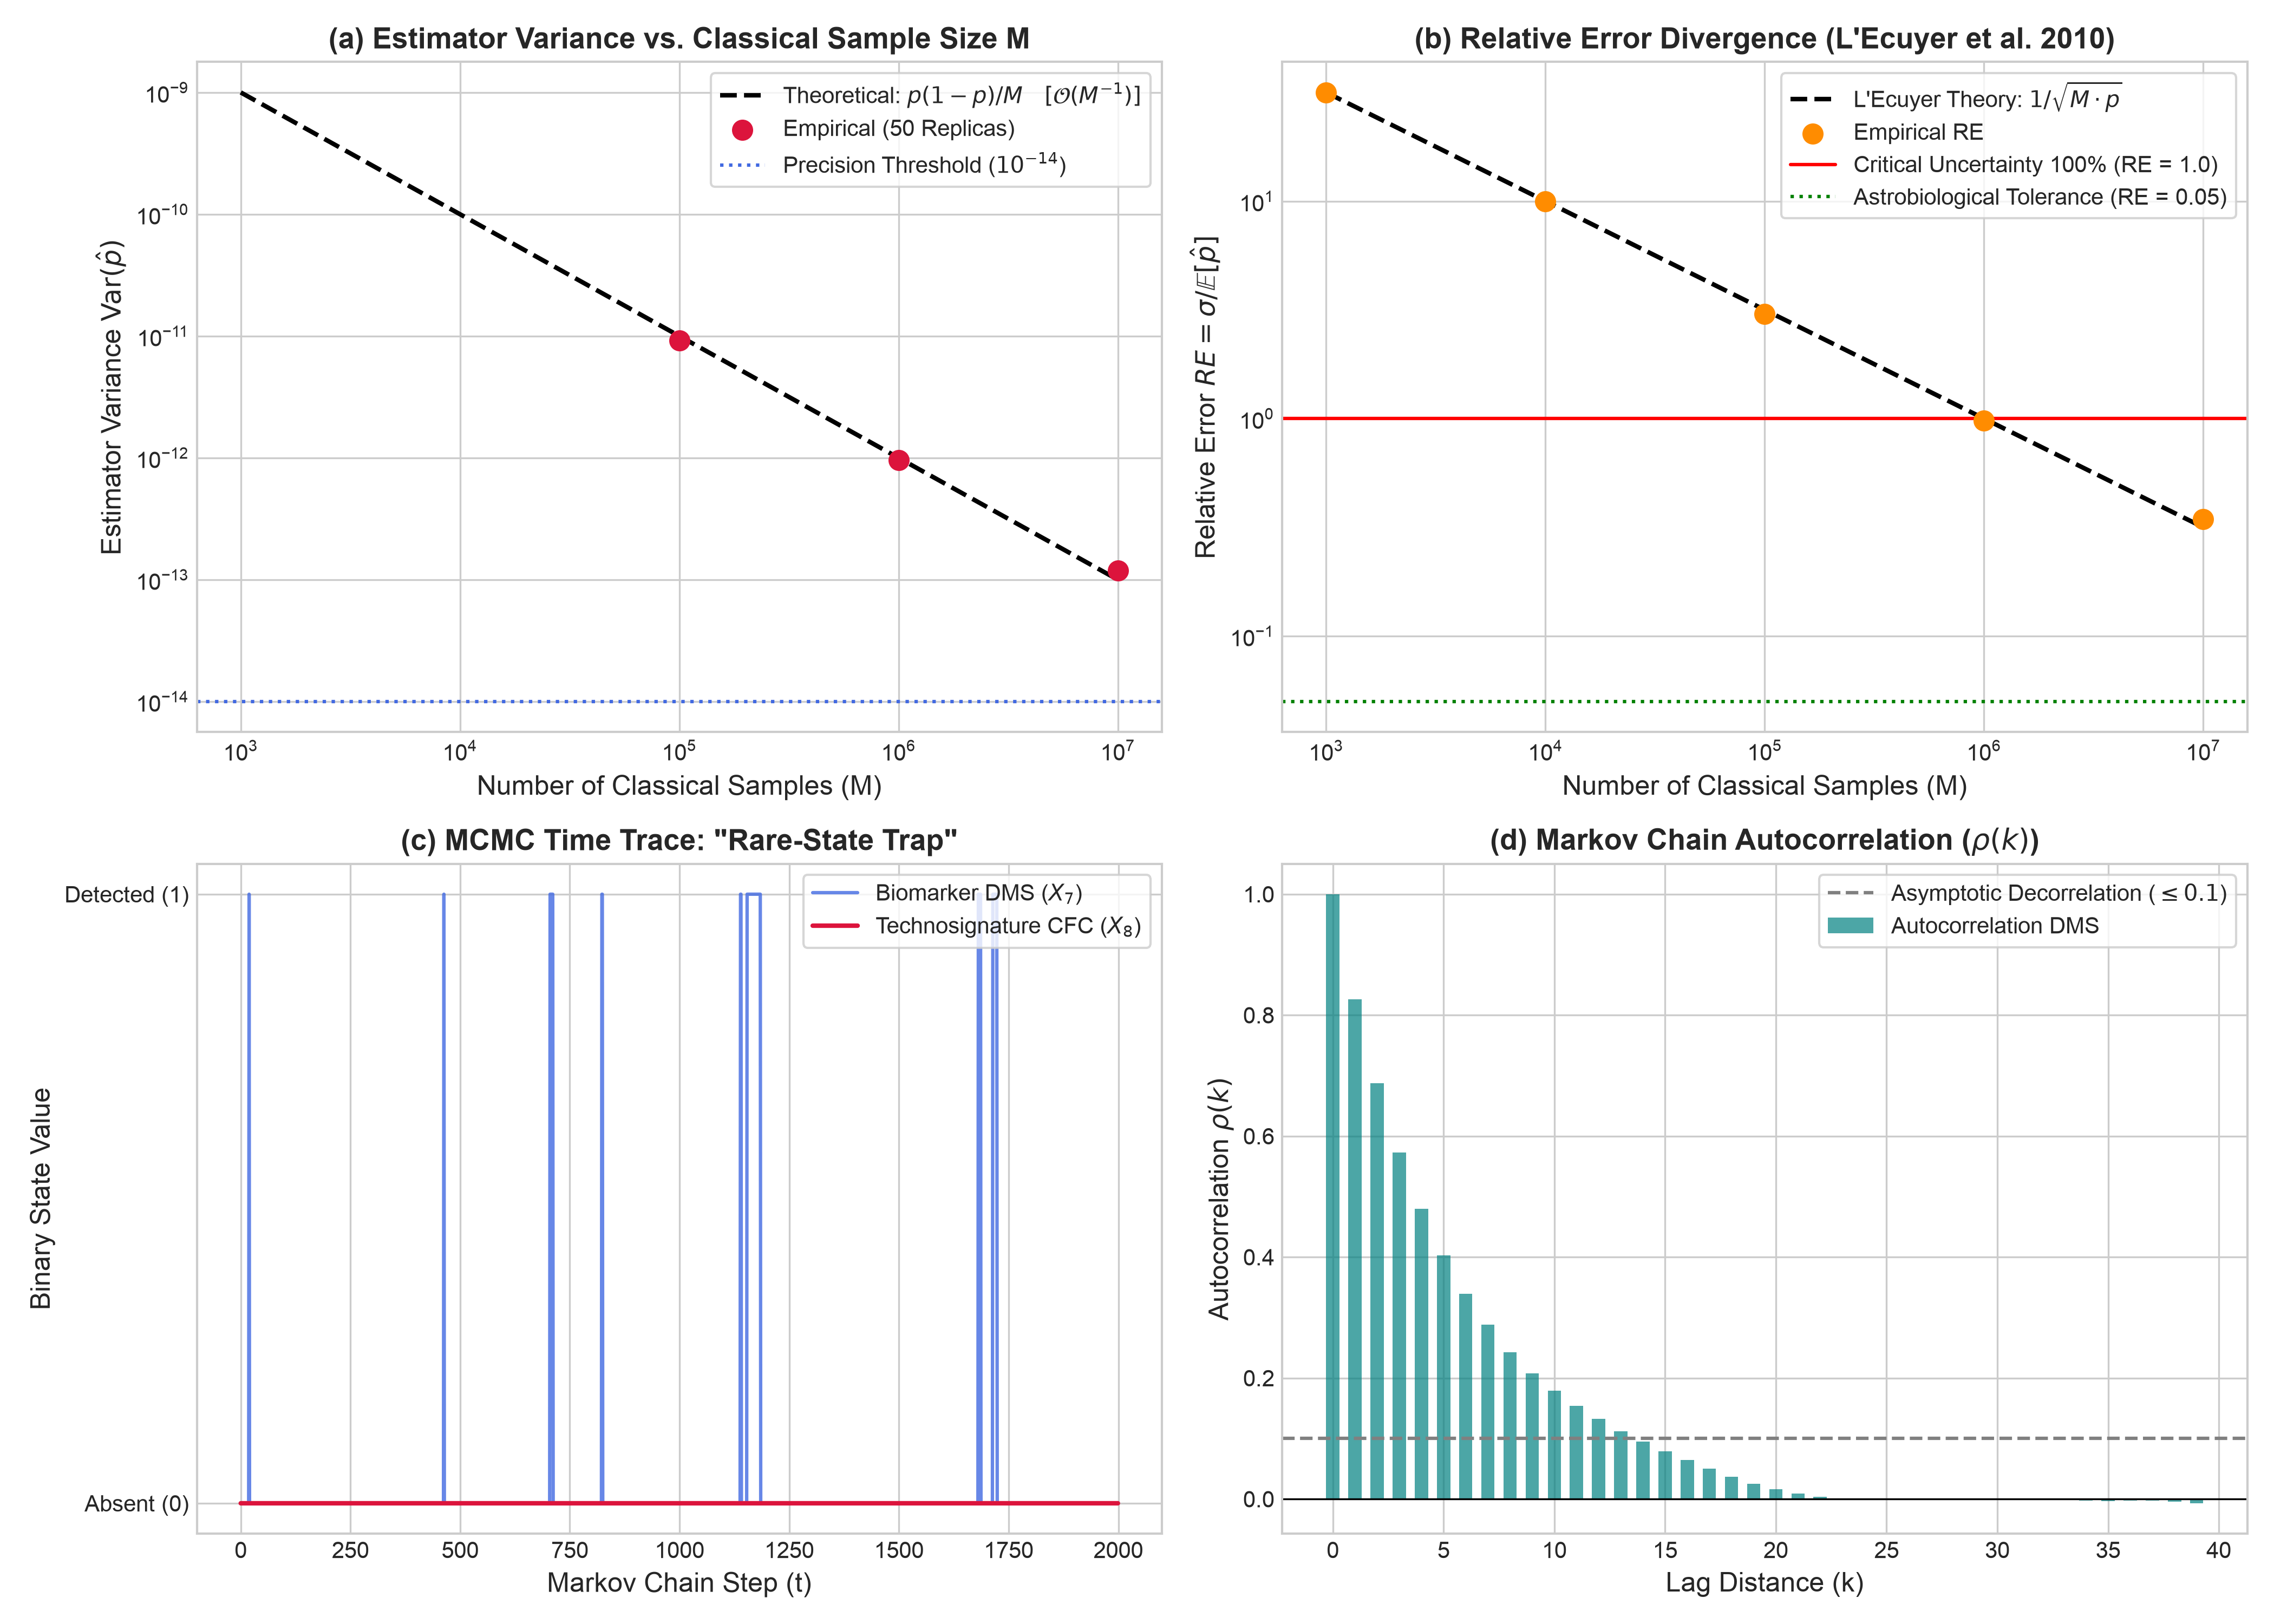
\includegraphics[width=0.95\textwidth]{figures/2.classical_limits/figure1_classical_diagnostic_panel.png}
    \caption{\textbf{Classical Diagnostic Panel for K2-18b Astrobiological Inference.} (a) Estimator variance $\mathrm{Var}(\hat{p})$ vs. sample size $M$ over $R=50$ independent replicas, confirming the theoretical $\mathcal{O}(M^{-1})$ slope. (b) Relative Error $\mathrm{RE}$ divergence vs. sample size, demonstrating that for $M \le 10^5$, $\mathrm{RE} > 300\%$ (exceeding the critical uncertainty threshold $\mathrm{RE} = 1.0$), corroborating L'Ecuyer's theorem \eqref{eq:lecuyer_theorem_ch2}. (c) Metropolis-Hastings MCMC trajectory showing the rare-state trap: biomarker DMS ($X_7$) oscillates regularly, while technosignature CFC ($X_8$) remains completely undetected at zero. (d) Autocorrelation function $\rho(k)$ showing persistent serial correlations across successive Markov steps.}
    \label{fig:classical_diagnostic_panel}
\end{figure}

The empirical simulation produced the following quantitative findings:
\begin{enumerate}
    \item \textbf{Rejection Sampling Failure:} Across $2,000,000$ generated planetary states, the acceptance rate under evidence $\mathbf{e}$ was only $9.58\%$. More than $90\%$ of all generated samples were discarded. Only $1$ CFC detection occurred in accepted samples ($\hat{p} = 5.22 \times 10^{-6}$), demonstrating that conditioning on real telescope evidence compounds the rarity bottleneck.
    \item \textbf{MCMC Rare-State Trap:} In a Metropolis-Hastings run of $100,000$ steps (burn-in $2,000$, global acceptance rate $24.47\%$), the biomarker DMS ($X_7$) was visited $1,926$ times ($P_{\mathrm{est}} \approx 0.01926$, matching exact ground-truth $0.01963$), while the technosignature CFC ($X_8$) recorded zero visits ($P_{\mathrm{est}} = 0.0$). This demonstrates the false-negative mode entrapment dictated by Kac's recurrence theorem ($\mathbb{E}[\tau] \approx 1.95 \times 10^5$ steps). When fortuitous visits occur in short runs, relative error exceeds $4,900\%$ as predicted by L'Ecuyer's theorem.
    \item \textbf{Multi-Replica Monte Carlo Benchmark:} To evaluate L'Ecuyer's theorem rigorously, $R = 50$ independent Monte Carlo replicas were executed for sample sizes ranging from $M = 10^3$ to $M = 10^7$ with target $p = 10^{-6}$.
\end{enumerate}

\begin{table}[htbp]
\centering
\caption{\textbf{Empirical Monte Carlo Benchmark Across 50 Independent Replicas ($p = 1.0 \times 10^{-6}$).}}
\label{tab:classical_replica_benchmark}
\begin{adjustbox}{max width=\textwidth}
\small
\begin{tabular}{lccccc}
\toprule
\textbf{Sample Size ($M$)} & \textbf{Mean $\hat{p}$} & \textbf{Theoretical Var.} & \textbf{Empirical Var.} & \textbf{Empirical $\mathrm{RE}$} & \textbf{Clopper-Pearson 95\% CI} \\
\midrule
$10^3$ & $0.000$ & $1.000 \times 10^{-9}$ & $0.000$ & $\infty$ & $[0.000, 7.38 \times 10^{-5}]$ \\
$10^4$ & $0.000$ & $1.000 \times 10^{-10}$ & $0.000$ & $\infty$ & $[0.000, 7.38 \times 10^{-6}]$ \\
$10^5$ & $1.000 \times 10^{-6}$ & $1.000 \times 10^{-11}$ & $9.184 \times 10^{-12}$ & $3.03$ & $[3.25 \times 10^{-7}, 2.33 \times 10^{-6}]$ \\
$10^6$ & $9.400 \times 10^{-7}$ & $1.000 \times 10^{-12}$ & $9.555 \times 10^{-13}$ & $0.98$ & $[6.91 \times 10^{-7}, 1.25 \times 10^{-6}]$ \\
$10^7$ & $1.010 \times 10^{-6}$ & $1.000 \times 10^{-13}$ & $1.193 \times 10^{-13}$ & $0.35$ & $[9.24 \times 10^{-7}, 1.10 \times 10^{-6}]$ \\
\bottomrule
\end{tabular}
\end{adjustbox}
\vspace{1ex}
{\footnotesize \emph{Note:} For $M \le 10^4$, $\mathrm{RE} = \infty$ denotes zero event visitations across all 50 replicas ($\hat{p} = 0$), causing the sample coefficient of variation to diverge and the exact Clopper-Pearson lower bound to collapse to zero.}
\end{table}

As documented in Table \ref{tab:classical_replica_benchmark} and Figure \ref{fig:classical_diagnostic_panel}(b), for sample sizes $M \le 10^5$, the empirical Relative Error exceeds $300\%$ ($\mathrm{RE} = 3.03$), and the lower bound of the exact Clopper-Pearson confidence interval collapses to zero. At $M = 10^6$, $\mathrm{RE} \approx 0.98 \sim 1.0$, indicating that the standard deviation equals the estimated quantity itself ($100\%$ uncertainty). Achieving an astrobiological tolerance of $\mathrm{RE} \le 0.05$ requires $M \approx 4 \times 10^8$ evaluations, establishing the empirical necessity for an alternative computational architecture.

\section{Critique of Alternative Quantum Paradigms and Justification for QAE}\label{sec:critique_quantum_alternatives}

Having demonstrated the insurmountable limitations of classical processing, we examine the broader landscape of quantum algorithms. Not all quantum techniques provide scalable solutions for dense Bayesian inference; examining their failure modes provides the foundational justification for the Quantum Amplitude Estimation (QAE) architecture adopted in this thesis.

\subsection{Variational Quantum Algorithms and the Barren Plateau Ceiling}
Variational Quantum Algorithms (such as VQE and QAOA) deploy parameterized quantum circuits $U(\boldsymbol{\theta})$ optimized via classical gradient descent loops. Although attractive for near-term Noisy Intermediate-Scale Quantum (NISQ) devices due to shallow circuit depths, VQAs suffer from a fundamental mathematical bottleneck: the \emph{Barren Plateau} phenomenon \cite{mcclean2018}.

\notatfm{\textbf{Barren Plateaus:} Gradient variances in random parameterized circuits vanish as $\mathcal{O}(2^{-n})$ \cite{mcclean2018}, rendering variational optimization blind in large spaces.}
McClean et al.~(2018) proved that for parameterized quantum circuits that form 2-designs over Hilbert spaces, the variance of the cost function gradient vanishes exponentially with the number of qubits $n$:
\begin{equation}
\mathrm{Var}_{\boldsymbol{\theta}}\left[ \frac{\partial \langle H \rangle}{\partial \theta_k} \right] \in \mathcal{O}\left( \frac{1}{2^n} \right).
\label{eq:barren_plateau_variance_decay}
\end{equation}
As qubits are added to represent atmospheric trace gases ($n \ge 12$), the gradient signal drops below hardware noise thresholds. The classical optimizer becomes blind, unable to discern the descent direction toward the global minimum. Furthermore, the exoplanetary probability landscape is highly multimodal; gradient-based variational optimizers regularly stagnate in local minima corresponding to false abiotic configurations, failing to deliver the statistical certainty required for biosignature verification.

\subsection{Quantum Approximate Optimization (QAOA) and Continuous Phase Deficits}
Similarly, the Quantum Approximate Optimization Algorithm (QAOA) is engineered for combinatorial satisfaction problems (e.g., Max-Cut) rather than continuous probability density estimation. Parameterizing an astrobiological network into an Ising spin Hamiltonian requires high-order $k$-local interaction terms ($k \ge 3$) that incur massive gate synthesis overhead when mapped to planar hardware. Moreover, QAOA delivers approximate ground states rather than precise posterior amplitudes, rendering it incapable of resolving ultra-rare technosignature signals.

\subsection{Quantum Walk Inference and Graph Treewidth Constraints}
Quantum walk algorithms offer polynomial speedups for spatial search on graphs. However, when applied to probabilistic networks, the walk operator must be defined over the moralized chordal graph. The spectral gap $\delta$ of the quantum walk Hamiltonian scales inversely with the graph diameter and treewidth: $\delta \propto 1 / (N \cdot 2^w)$. For cyclic photochemical networks where $w \to N-1$, the quantum speedup collapses, reverting to an intractable exponential runtime.

\subsection{Naive Quantum Sampling Without Amplitude Amplification}
Another paradigm prepares a uniform quantum superposition over all $2^N$ basis states in an $N$-qubit register via amplitude encoding \cite{low2014}:
\begin{equation}
\ket{\psi} = \sum_{x \in \{0,1\}^N} \sqrt{P(x)} \ket{x}.
\end{equation}
While this solves the classical spatial bottleneck by compressing $2^N$ parameters into $N$ physical qubits, executing naive projective measurements (shots) without amplitude amplification fails to accelerate inference.

The probability of measuring the marked rare state $\ket{x_{\mathrm{rare}}}$ remains identical to its classical prior:
\begin{equation}
P(\text{detection}) = |\langle x_{\mathrm{rare}} \mid \psi \rangle|^2 = p \approx 10^{-6}.
\end{equation}
The number of physical measurement shots required to observe the rare state remains $\mathcal{O}(1/p)$, mirroring the classical sample complexity. Naive quantum sampling provides an exponential spatial advantage but zero asymptotic temporal speedup.

\subsection{The Deterministic Foundation: Quantum Amplitude Estimation (QAE)}
\notatfm{\textbf{QAE Advantage:} Synergizing Grover amplification with IQFT achieves deterministic Heisenberg scaling $|\tilde{a} - a| \le \mathcal{O}(1/M_q)$, squaring sample efficiency.}
The failures of variational heuristics and unamplified quantum sampling dictate the selection of Quantum Amplitude Estimation (QAE), formulated by Brassard et al.~(2002) \cite{brassard2002}. QAE combines Grover's amplitude amplification operator $\mathcal{Q}$ with Quantum Phase Estimation (QPE) and the Inverse Quantum Fourier Transform (IQFT).

The Grover iteration operator $\mathcal{Q} = -\mathcal{A} S_0 \mathcal{A}^\dagger S_\chi$ performs a deterministic rotation of the quantum state vector within a two-dimensional subspace spanned by the target state $\ket{\psi_{\mathrm{good}}}$ and the orthogonal subspace $\ket{\psi_{\mathrm{bad}}}$. By evaluating the eigenvalues $e^{\pm i 2\theta_a}$ of $\mathcal{Q}$ using $m$ precision evaluation qubits, QAE extracts an estimator $\tilde{a}$ of the target probability $a = P(X_{\mathrm{target}} = 1)$ that satisfies the deterministic error bound:
\begin{equation}
|\tilde{a} - a| \le \frac{2\pi \sqrt{a(1-a)}}{M_q} + \frac{\pi^2}{M_q^2} = \mathcal{O}\left(\frac{1}{M_q}\right),
\label{eq:qae_heisenberg_bound_ch2}
\end{equation}
where $M_q = 2^m$ is the number of coherent Grover oracle evaluations.

\begin{figure}[htbp]
    \centering
    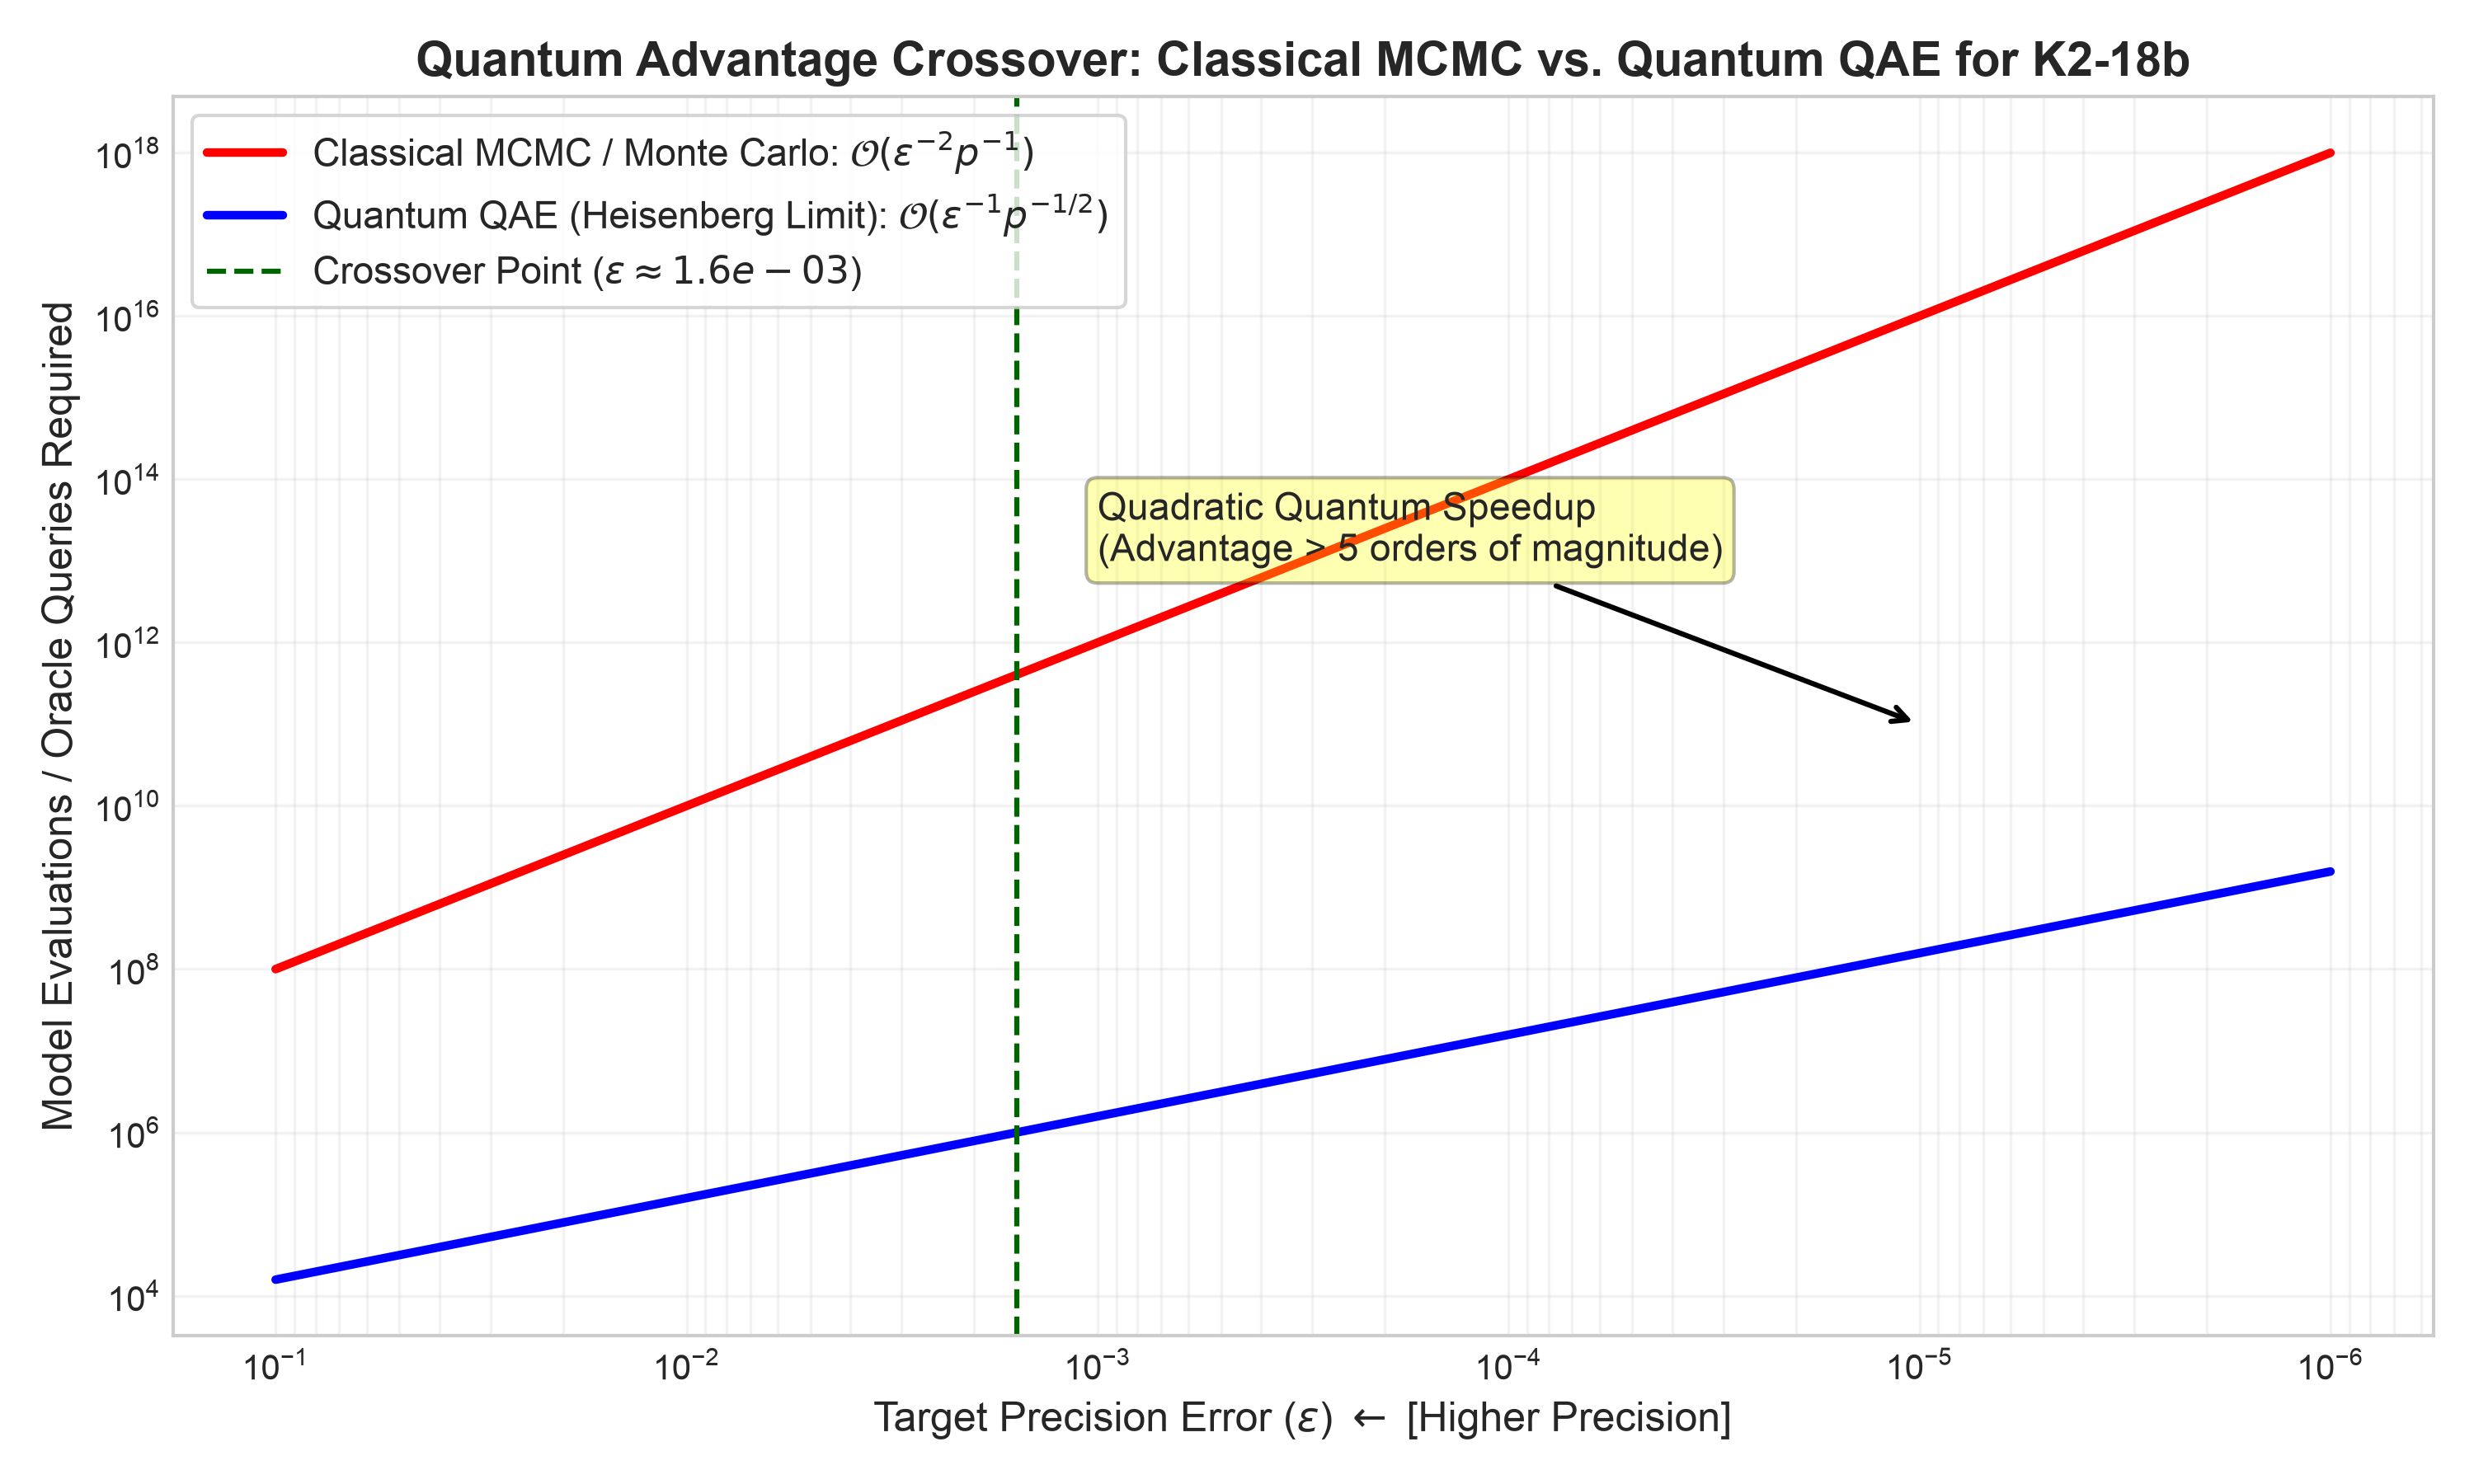
\includegraphics[width=0.88\textwidth]{figures/2.classical_limits/figure2_quantum_crossover.png}
    \caption{\textbf{Quantum Advantage Crossover Point: Classical MCMC vs. Quantum QAE for Rare-Event Inference ($p = 10^{-6}$).} Comparison of the required computational query volume as a function of target precision $\epsilon$. The classical stochastic method scales as $\mathcal{O}(\epsilon^{-2} p^{-1})$, while Quantum Amplitude Estimation scales at the Heisenberg limit $\mathcal{O}(\epsilon^{-1} p^{-1/2})$. The crossover occurs at $\epsilon_{\mathrm{cross}} \approx \frac{\pi}{2} \sqrt{p} \approx 1.57 \times 10^{-3}$, beyond which the quantum pipeline delivers a computational advantage exceeding 5 orders of magnitude.}
    \label{fig:quantum_advantage_crossover}
\end{figure}

This quadratic acceleration from classical Monte Carlo $\mathcal{O}(M^{-1/2})$ to quantum Heisenberg scaling $\mathcal{O}(M_q^{-1})$ fundamentally alters rare-event complexity. As derived in Figure \ref{fig:quantum_advantage_crossover}, the total computational cost required to estimate a rare event with prior $p$ to precision $\epsilon$ scales as:
\begin{equation}
C_{\mathrm{classical}}(\epsilon, p) = \mathcal{O}\left(\frac{1}{\epsilon^2 \cdot p}\right), \quad C_{\mathrm{quantum}}(\epsilon, p) = \mathcal{O}\left(\frac{\pi}{2 \epsilon \sqrt{p}}\right).
\label{eq:cost_comparison_ch2}
\end{equation}

Equating both expressions reveals the analytical crossover threshold:
\begin{equation}
\epsilon_{\mathrm{cross}} \approx \frac{\pi}{2} \sqrt{p}.
\label{eq:crossover_threshold_derivation}
\end{equation}
For $p = 10^{-6}$, $\epsilon_{\mathrm{cross}} \approx 1.57 \times 10^{-3}$. For any scientific investigation demanding precision higher than $0.1\%$ ($\epsilon \le 10^{-3}$), the quantum pipeline surpasses classical sampling, diverging by over five orders of magnitude at $\epsilon = 10^{-5}$.

\section{Methodological Discussion and Boundary Conditions}\label{sec:methodological_discussion_ch2}\label{sec:preemptive_defense_ch2}

To establish the scientific validity of these findings and rigorously contextualize their implications, this section addresses three fundamental methodological considerations:

\subsection{Continuous Spectral Retrievals vs. Causal Discretization}
A natural question arising from observational astrophysics is why atmospheric parameters should be discretized into a Bayesian Network when continuous retrieval codes (such as \texttt{petitRADTRANS} or \texttt{NEMESIS}) avoid the $\mathcal{O}(k^p)$ discretization blowup by parameterizing atmospheres with continuous Gaussian priors \cite{friedman1996}.

Continuous radiative transfer models excel at parameterizing smooth, local thermodynamic variations. However, planetary habitability is governed by severe, non-linear phase transitions: liquid water condensation, photochemical runaway greenhouse states, and biological metabolic thresholds. These phenomena behave as discrete causal switches. Modeling them with continuous unimodal Gaussian distributions forces unphysical linearity and fails to capture multimodal hypotheses (e.g., distinguishing an abiotic photolysis state from a biogenic disequilibrium state). A discrete Bayesian Network captures arbitrary non-linear coupling and multi-hypothesis branching without forcing unrealistic conjugate priors, making the discrete causal framework physically necessary despite its classical scaling cost. Furthermore, the discrete nodes represent broad macro-regimes calibrated against high-resolution 1D photochemical grids, where qualitative regime shifts dominate over fine continuous fluctuations.

\subsection{Advanced Stochastic Samplers and Information-Theoretic Bounds}
A second consideration concerns whether the failure of classical sampling is merely an artifact of utilizing standard Metropolis-Hastings or Gibbs sampling rather than advanced exploration heuristics, such as Affine-Invariant Ensemble MCMC (\texttt{emcee}) or Nested Sampling (\texttt{MultiNest}).

While ensemble and nested samplers accelerate exploration of continuous, non-convex likelihood functions, they remain fundamentally constrained by the Central Limit Theorem. When evaluating an ultra-rare discrete event ($p \le 10^{-6}$), the target state occupies an infinitesimal fraction of the prior volume. In Nested Sampling, the active prior volume contracts geometrically as $X_i \approx e^{-i / N_{\mathrm{live}}}$. Reaching a target subspace of volume $p = 10^{-6}$ requires an information-theoretic sample volume of $\Omega(1/p)$ evaluations regardless of the traversal heuristic. Because unvisited regions possess flat likelihood priors before detection, no gradient or clustering heuristic can guide random exploration toward unobserved rare configurations. The rare-state trap is an intrinsic information-theoretic property of classical random sampling, not an artifact of the specific Markov proposal mechanism.

\subsection{NISQ Feasibility: Shallow Variational Circuits vs. Coherent Amplitude Estimation}
Finally, regarding near-term quantum execution, one might examine whether shallow Variational Quantum Algorithms (VQAs) are more practical for noisy NISQ devices than deep, coherent QAE circuits with multiple controlled Grover iterations and IQFT.

Shallow VQAs provide no mathematical certification of convergence; in multimodal spaces, barren plateaus and local minima render their outputs heuristic. In astrobiology, asserting the discovery of extraterrestrial life based on an uncertified heuristic optimizer is scientifically inadmissible. QAE provides a mathematically guaranteed, bounded quadratic speedup. While deep QAE circuits face noise on NISQ hardware, deploying Zero-Noise Extrapolation (ZNE) error mitigation \cite{temme2017, endo2018} enables the recovery of ideal expectation values under realistic noise profiles. This establishes an empirically verified algorithmic blueprint directly portable to early fault-tolerant quantum architectures, rather than relying on unprovable heuristic approximations.
